\section{Method}
\label{sec:method}

\subsection{Dataset}

The dataset we are using is the Pima Indians Diabetes Database. It is a dataset that is used to benchmark many machine learning algorithms. There are 8 features and 1 ouput. The features are the number of pregnancies, glucose concentration, blood pressure, skin thickness, insulin, body mass index, diabetes pedigree function and age. The output is a binary value of 1 or 0 indicating if the patient has diabetes or not. The goal with this dataset is to predict if a patient has diabetes or not based on the features \cite{Kaggle_Pima_Indians}.

Upon inspection of the dataset we found that there were some missing or invalid values. There were 0 values for many of the features which is not possible for a living person. We chose a simple way to handle this which was to replace these values with the mean of the feature. This lets all the samples be kept but will reduce the variance of the dataset \cite{GFG_Missing_Values}.

We chose to use standardisation(z-score) to scale the features since the features since the features have different units and scales. Standardisation is better suited than min-max normalisation since it handles outliers better and doesn't constrain the scaled values to a specific range \cite{GFG_Data_Normalization}. This is important since there could be outliers in the dataset or in future datasets that we use the model on.

It was also found that the dataset is imbalanced. There are 500 samples without diabetes and 268 samples with diabetes. This was important to consider when training and evaluating the models. 

\subsection{Evaluation}

The models are evaluated using stratified 8-fold cross-validation. Using cross-validation helps better estimate the performance of the models on unseen data that using a single train-test split. Stratified cross-validation is used since the dataset is imbalanced and ensures that the class distribution is the same in each fold. This is important since we want to make sure that the model is learning from both classes equally and is not biased. $k=8$ was chosen since it divides the dataset eqaully. With 768 samples we get 96 samples in each fold \cite{Brownlee2023, Krasnoshchek2024, Brownlee2020_imbalanced, Psteen2020}.

To compare the models and variations we use the F1 score, accuracy, precision and recall metrics. Where $TP$ is the number of true positives, $TN$ is the number of true negatives, $FP$ is the number of false positives and $FN$ is the number of false negatives. \cite{Marsland2015}

\vspace{0.2cm}

\begin{itemize}
  \item \textbf{Accuracy}: The proportion of correct predictions among the total number of predictions.
  \begin{equation}
      \text{Accuracy} = \frac{TP + TN}{TP + TN + FP + FN}
  \end{equation}

  \item \textbf{Precision}: The proportion of correct positive predictions among all(correct and incorrect) positive predictions.
  \begin{equation}
      \text{Precision} = \frac{TP}{TP + FP}
  \end{equation}

  \item \textbf{Recall} The proportion of correct positive predictions among all actual positives.
  \begin{equation}
      \text{Recall} = \frac{TP}{TP + FN}
  \end{equation}

  \item \textbf{F1 Score}: The harmonic mean of precision and recall.
  \begin{equation}
      \text{F1 Score} = 2 \times \frac{\text{Precision} \times \text{Recall}}{\text{Precision} + \text{Recall}}
  \end{equation}
\end{itemize}

The F1 score was chosen since it is a good metric for imbalanced datasets since it considers both precision and recall. The precision and recall are also used since they give more insight into the trade-off between false positives and false negatives. The accuracy is also used since it is a good metric to give an overall view of the model's performance \cite{Brownlee2020_imbalanced_metrics}. Since 8-fold cross-validation is used the mean and standard deviation of the metrics will be used to compare the models.

Precision-Recall Curves(PR Curve) will also be used to compare the the cross-validation folds and the models. The area under the curve is also calculated. The PR curve is used since it is more informative than the ROC curve when dealing with imbalanced datasets. It will show how well the models classify compared to a random classifier across a range of thresholds \cite{scikit_learn_precision_recall}.

PR curves will be plotted for each fold as well as the mean PR curve. The area under the curve will be calculated for each fold and the mean area under the curve will be calculated. This will provide another good indication of how well the models are performing.

\subsection{Baseline Model}

% class BasePerceptron():
%     weights: torch.Tensor
%
%     def __init__(self, size: int):
%         self.weights = torch.zeros(size)
%
%     def update(self, learning_rate: float, dataset: Dataset):
%         for xi, yi in dataset:
%             y_mapped = 2 * yi - 1
%             cond = y_mapped * torch.dot(xi, self.weights)
%             if cond <= 0:
%                 self.weights += learning_rate * y_mapped * xi
%
%     def predict_prob(self, new_X: torch.Tensor):
%         return torch.dot(new_X, self.weights)
%
%     def predict(self, new_X: torch.Tensor):
%         return 1 if self.predict_prob(new_X) >= 0 else 0

The baseline perceptron model that was implemented is a simple linear classifer. It learns from a dataset by updating it's weights based on the samples in the dataset. The output of the model is a binary value of 1 or 0 allowing it to be used for binary classification \cite{Marsland2015}. 

The model is initialised with a weights vector of zeros. The size of the weights vector is the same as the number of features in the dataset. Our version uses an activation function similar to the sign function. Our activation functi $f(z)$ ensures that the training does not get stuck when the weights 0. The activation function is defined as:

\[
f(z) = 
\begin{cases} 
1 & \text{if } z \geq 0 \\ 
0 & \text{if } z < 0 
\end{cases}
\]

\subsubsection{Training}

The training process involves iterating over the dataset and updating the weights $\boldsymbol{w}$ based on the samples in the dataset. The learning rate $\eta$ is a hyperparameter that controls how much the weights are updated. The loss function $l_i$ is used to calculate how far the prediction is from the correct output. In this case the loss function is the perceptron loss function. With this loss function the weights are only updated if the prediction is incorrect. The weights are updated using the following process \cite{Marsland2015}:

\begin{algorithm}
  \caption{Baseline Perceptron Learning Algorithm}
  \begin{algorithmic}
    \State $\boldsymbol{w} \gets \text{initialise to zeros}$
    \For{$\boldsymbol{x}_i, y_i$ in training dataset}
      \State $y^* \gets f(\boldsymbol{x}_i \cdot \boldsymbol{w})$
      \State $l_i \gets \max\{0, -y_i \langle \boldsymbol{x_i}, \boldsymbol{w} \rangle\}$
      \State $\boldsymbol{w} \gets \boldsymbol{w} + \eta \cdot l_i \cdot \boldsymbol{x}_i$
    \EndFor
  \end{algorithmic}
\end{algorithm}

\subsubsection{Prediction}

The prediction process involves taking the dot product of the input features $\boldsymbol{x}$ and the weights $\boldsymbol{w}$. This is then passed through the activation function to get the output $y$. The output is then used to classify the input features into one of the classes. The decision function is defined as:

\[
  y = f(\boldsymbol{x} \cdot \boldsymbol{w})
\]

\subsubsection{Constraints}

Single layer perceptrons are only able to learn linear decision boundaries. This means that the model will only be able to classify the data if it is linearly separable. If the data is not linearly separable the model will not be able to learn a decision boundary that can classify the data. 


\subsection{Baseline w/ Bias}

The baseline model does not include a bias term. Adding a bias term allows the decision boundary to move away from the origin. This allows the model to learn a better decision boundary and improve the performance of the model. 
To avoid have to change the baseline model implementation too much, the bias term is added as an extra weight to the weights vector. An additional input is also added to the input vector which is always 1. This works because \cite{Marsland2015}:

\begin{equation}
  \boldsymbol{w} = [w_1, w_2, \ldots, w_n, b]
\end{equation}
\begin{equation}
  \boldsymbol{x_i} = [x_{i1}, x_{i2}, \ldots, x_{in}, 1]
\end{equation}
\begin{equation}
  \boldsymbol{w} \cdot \boldsymbol{x_i} = \sum_{j=1}^{n} w_j \cdot x_{ij} + b \cdot 1
\end{equation}

\subsection{L2 Regularisation}

L2 regularisation is added to the model to help prevent overfitting. L2 regularisation adds a penalty term to the loss function that is proportional to the square of the weights. This will help prevent the weights from becoming too large and overfitting the training data. The regularisation term is added to the weight update step.

\begin{equation}
  \boldsymbol{w} \gets \boldsymbol{w} - \eta \cdot l_i \cdot \boldsymbol{x}_i - \lambda \cdot \boldsymbol{w}
\end{equation}

\subsection{Class Weighting}

% def calc_class_weights(dataset):
%     class_counts = [0, 0]
%     for _, yi in dataset:
%         class_counts[int(yi)] += 1
%
%     class_weight_0 = len(dataset) / (class_counts[0] * 2)
%     class_weight_1 = len(dataset) / (class_counts[1] * 2)
%     print(f"Class weights: {class_weight_0}, {class_weight_1}")
%
%     return class_weight_0, class_weight_1

Since the dataset is imbalanced we attempted using class weighting to mitigate any possibilities of the model being biased towards the majority class. 
The class weights are calculated by taking the total number of samples and dividing it by twice the number of samples in each class. This gives a higher weight to the minority class. The class weights are then used in the loss function to give more importance to the minority class \cite{Abhinav2023}.

Class weights are calculated and used as follows:

\begin{equation}
  \text{class\_weight} = \frac{\text{total samples}}{2 \times \text{class samples}}
\end{equation}

\begin{equation}
  l_i = \max\{0, -y_i \langle \boldsymbol{x_i}, \boldsymbol{w} \rangle\} \cdot \text{class\_weight}
\end{equation}


\subsection{Gradient Descent w/ Sigmoid Activation}

% class PerceptronWithGD():
%     weights: torch.Tensor
%
%     def __init__(self, size: int, l2_lambda=0.01, class_weights=(1, 1), activation=torch.sigmoid):
%         self.weights = torch.randn(size)
%         self.b = 0
%         self.l2_lambda = l2_lambda
%         self.class_weights = class_weights
%         self.activation = activation
%
%     def update(self, learning_rate: float, dataset: Dataset):
%         X = torch.stack([xi for xi, yi in dataset])
%         y = torch.tensor([yi for xi, yi in dataset])
%
%         comb = torch.matmul(X, self.weights) + self.b
%
%         y_pred = self.activation(comb)
%
%         diff = y - y_pred
%
%         weighted_diff = torch.where(
%             y == 1, diff * self.class_weights[1], diff * self.class_weights[0])
%
%         regularization_term = 2 * self.l2_lambda * self.weights
%
%         self.weights += learning_rate * \
%             (torch.matmul(X.T, weighted_diff) - regularization_term)
%         self.b += learning_rate * torch.sum(weighted_diff)

The next step was to move away from the Perceptron learning algorithm and move towards a more generalised learning algorithm. We chose to use gradient descent with a sigmoid activation function. The sigmoid activation function is used since it is a good activation function for binary classification problems.

The sigmoid activation function is defined as:

\begin{equation}
  f(z) = \frac{1}{1 + e^{-z}}
\end{equation}

The output of the model is then passed through the sigmoid activation function to get the output $y$. The output is then used to classify the input features into one of the classes. 

The new training process involves calculating the output of the model using the sigmoid activation function. The loss function is then calculated using the output of the model and the correct output. The weights are then updated based on the loss function. 

\section{Experiments}

\subsection{Baseline}

A learning rate of 0.01 and 200 epochs was used as a starting point for the baseline model. Increasing the learning rate just made the learning more unstable where as decreasing the learning rate did not really have any effect.

The results of the baseline Perceptron model(Table \ref{tab:cv_metrics}) were a good starting point. With a mean accuracy of 0.70 and a mean F1 score of 0.62 it performs better than a random classifer, but still leaves plenty of room for improvement. The PR curve in Figure \ref{fig:baseline_pr} also shows that the model is performing better than a random classifier.

\begin{table}[ht!]
    \centering
    \begin{tabular}{lcc}
        \toprule
        \textbf{Metric} & \textbf{Mean} & \textbf{Standard Deviation} \\
        \midrule
        Accuracy & 0.70 & 0.04 \\
        F1 Score & 0.62 & 0.08 \\
        Recall & 0.70 & 0.10 \\
        Precision & 0.56 & 0.07 \\
        Mean PR AUC & 0.65 & - \\
        \bottomrule
    \end{tabular}
    \caption{Baseline Perceptron Cross-Validation Metrics}
    \label{tab:cv_metrics}
\end{table}

\begin{figure}[ht!]
    \centering
    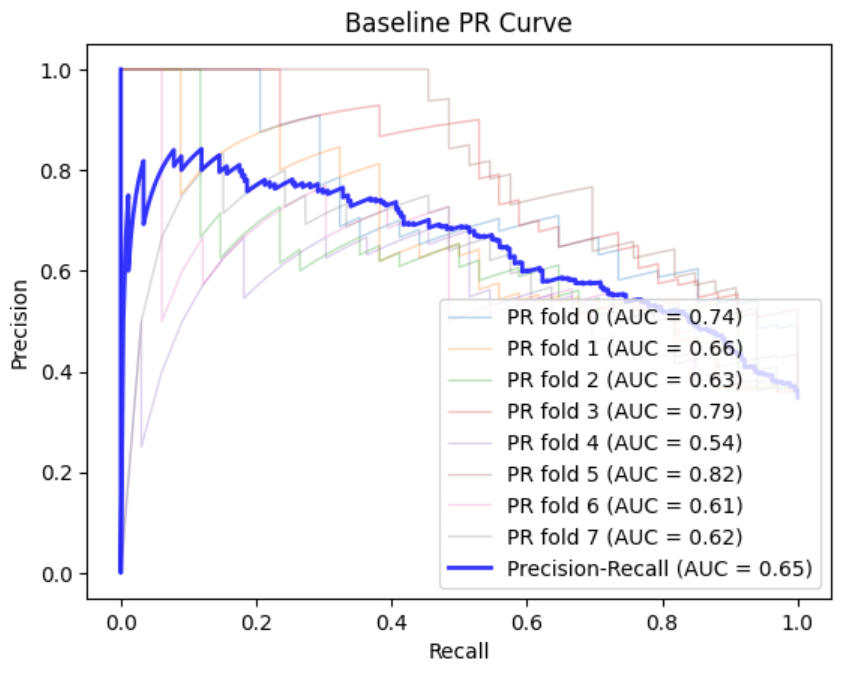
\includegraphics[width=0.5\textwidth]{images/baseline_pr.png}
    \caption{Baseline Perceptron PR Curve. Each point is a different threshold.}
    \label{fig:baseline_pr}
\end{figure}

The baseline model converges very quickly after roughly 10 epochs which can be seen in Figure \ref{fig:baseline_train_acc}. This is likely due to the simplicity of the dataset and the model. The model is able to learn a decision boundary quickly and does not need many epochs to do so. 

\begin{figure}[ht!]
    \centering
    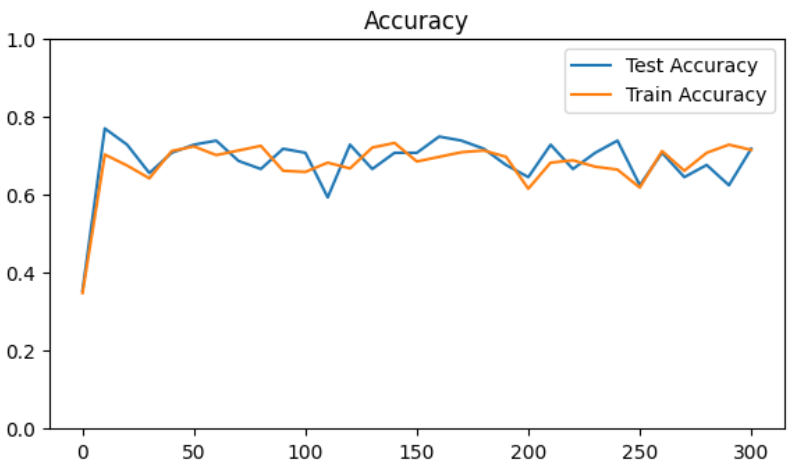
\includegraphics[width=0.5\textwidth]{images/baseline_train_acc.png}
    \caption{Baseline Perceptron training accuracy for fold 0.}
    \label{fig:baseline_train_acc}
\end{figure}

Since our baseline model does not include a bias term, the decision boundary will always pass through the origin. The obvious next step is to add a bias term to the model to allow the decision boundary to move away from the origin. This should allow the model to learn a better decision boundary and improve the performance of the model.

\subsection{Baseline w/ Bias}

The bias term is added as an extra weight to the weights vector. Then an additional input is added to the input vector which is always 1. The bias is added this way to make it compatible with the current baseline model implementation. The bias term is updated in the same way as the other weights.

Adding a bias term in theory should let the model learn a better decision boundary as it lets the decision bounday move away from the origin.

The results of adding a bias term(Table \ref{tab:bias_metrics}) were not as expected. The model performed worse than the baseline model. The mean accuracy was 0.70 and the mean F1 score was 0.56. The PR curve in Figure \ref{fig:bias_pr} shows that the model is performing worse than the baseline model. The mean PR AUC was also lower than the baseline model.

\begin{table}[ht!]
    \centering
    \begin{tabular}{lcc}
        \toprule
        \textbf{Metric} & \textbf{Mean} & \textbf{Standard Deviation} \\
        \midrule
        Accuracy & 0.70 & 0.07 \\
        F1 Score & 0.56 & 0.09 \\
        Recall & 0.54 & 0.10 \\
        Precision & 0.59 & 0.11 \\
        Mean PR AUC & 0.61 & - \\
        \bottomrule
    \end{tabular}
    \caption{Bias Perceptron Cross-Validation Metrics}
    \label{tab:bias_metrics}
\end{table}

\begin{figure}[ht!]
    \centering
    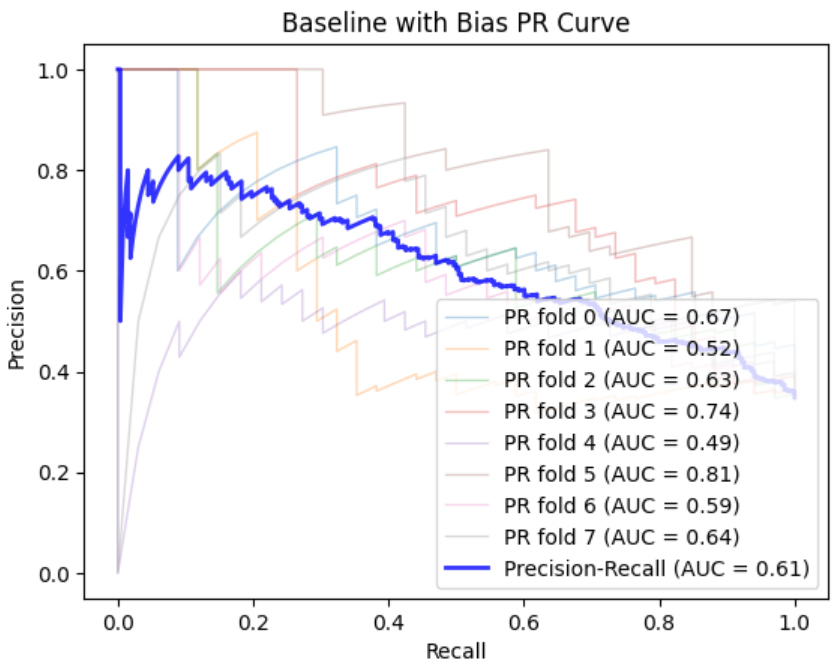
\includegraphics[width=0.5\textwidth]{images/bias_pr.png}
    \caption{Bias Perceptron PR Curve.}
    \label{fig:bias_pr}
\end{figure}

The reduction in performance from adding the bias term is likely from overfitting. Now that the decision boundary is not constrained to pass through the origin it can more closely fit the training data. One way to combat this is to add L2 regularisation to the model. 
  

\subsection{Baseline w/ Bias and L2 Regularisation}

L2 regularisation is added to the model to help prevent overfitting. L2 regularisation adds a penalty term to the loss function that is proportional to the square of the weights. This will help prevent the weights from becoming too large and overfitting the training data. The regularisation term is added to the weight update step.

Making $\lambda$ too large caused the accuracy to oscillate and the overall performance to decrease. A $\lambda$ of 0.01 was chosen since it gave the best performance. The results(Table \ref{tab:reg_metrics}) only slightly better than Baseline w/ Bias although precision was slightly lower. This potentially indicated that the model's current design was not able to learn a better decision boundary.

\begin{table}[ht!]
    \centering
    \begin{tabular}{lcc}
        \toprule
        \textbf{Metric} & \textbf{Mean} & \textbf{Standard Deviation} \\
        \midrule
        Accuracy & 0.70 & 0.02 \\
        F1 Score & 0.57 & 0.07 \\
        Recall & 0.57 & 0.13 \\
        Precision & 0.58 & 0.05 \\
        Mean PR AUC & 0.61 & - \\
        \bottomrule
    \end{tabular}
    \caption{L2 Regularisation Perceptron Cross-Validation Metrics}
    \label{tab:reg_metrics}
\end{table}

\begin{figure}[ht!]
    \centering
    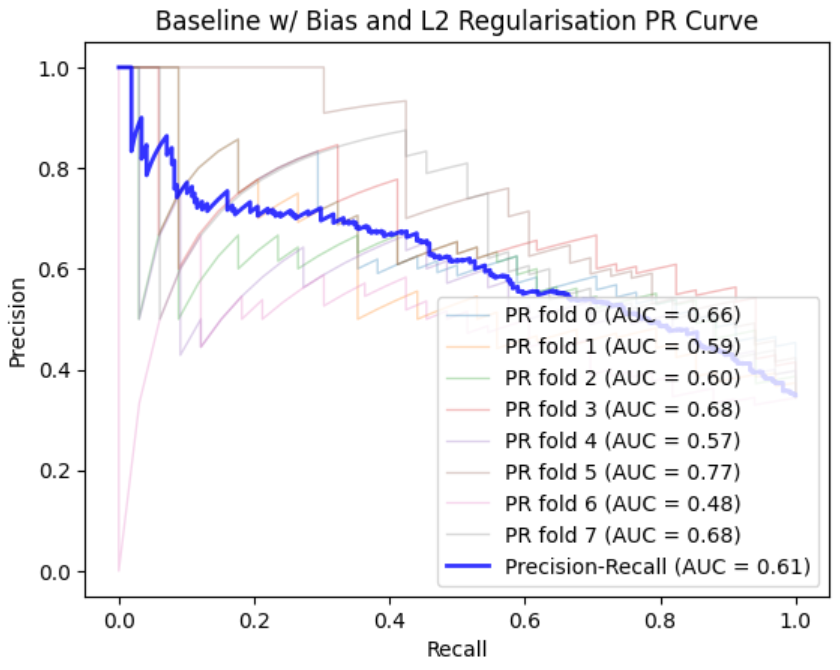
\includegraphics[width=0.5\textwidth]{images/reg_pr.png}
    \caption{Baseline w/ L2 Regularisation Perceptron PR Curve.}
    \label{fig:reg_pr}
\end{figure}


\subsection{Baseline w/ Bias and Class Weighting}

Since the dataset is imbalanced we attempted using class weighting to mitigate any possibilities of the model being biased towards the majority class. Since the positive class is the minority class, giving it a higher weight than the negative class should help the model learn from the positive class more. 

The results of adding class weighting(Table \ref{tab:weight_metrics}) were good. While the accuracy decreased slightly, the F1 score increased. This is due to the recall significantly increasing. This shows that the model did improve it's ability  to classify the positive class. The PR curve in Figure \ref{fig:weight_pr} also shows that the model is performing slightly better than the baseline w/ bias model.

\begin{table}[ht!]
    \centering
    \begin{tabular}{lcc}
        \toprule
        \textbf{Metric} & \textbf{Mean} & \textbf{Standard Deviation} \\
        \midrule
        Accuracy & 0.68 & 0.05 \\
        F1 Score & 0.60 & 0.09 \\
        Recall & 0.72 & 0.14 \\
        Precision & 0.53 & 0.07 \\
        Mean PR AUC & 0.62 & - \\
        \bottomrule
    \end{tabular}
    \caption{Class Weighting Perceptron Cross-Validation Metrics}
    \label{tab:weight_metrics}
\end{table}

\begin{figure}[ht!]
    \centering
    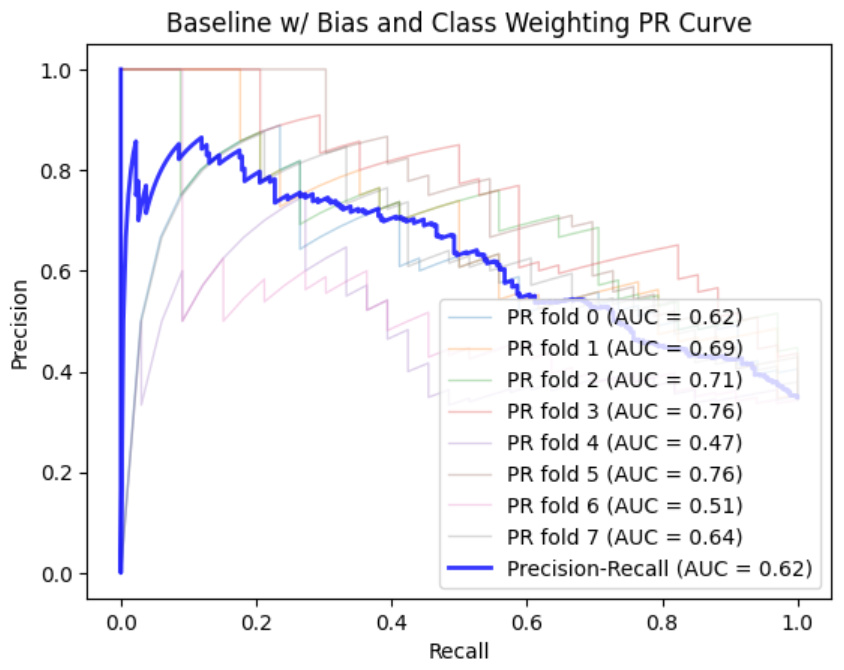
\includegraphics[width=0.5\textwidth]{images/class_weighting_pr.png}
    \caption{Class Weighting Perceptron PR Curve.}
    \label{fig:weight_pr}
\end{figure}

\subsection{Gradient Descent w/ Sigmoid Activation}

The next step was to move away from the Perceptron learning algorithm and move towards a more generalised learning algorithm. We chose to use gradient descent with a sigmoid activation function. The sigmoid activation function is used since it is a good activation function for binary classification problems. 

Other features the new design includes are a bias term, L2 regularisation and class weighting. A smaller learning rate of 0.001 was found to perform slightly better than the previous models. The results(Table \ref{tab:gd_metrics}) were a significant improvement over the previous models. The mean accuracy was 0.75 and the mean F1 score was 0.67. The PR curve in Figure \ref{fig:gd_pr} shows that the model is performing better than the previous models. The mean PR AUC is also the highest of all the models.

\begin{table}[ht!]
    \centering
    \begin{tabular}{lcc}
        \toprule
        \textbf{Metric} & \textbf{Mean} & \textbf{Standard Deviation} \\
        \midrule
        Accuracy & 0.75 & 0.05 \\
        F1 Score & 0.67 & 0.07 \\
        Recall & 0.72 & 0.08 \\
        Precision & 0.62 & 0.07 \\
        Mean PR AUC & 0.71 & - \\
        \bottomrule
    \end{tabular}
    \caption{Gradient Descent w/ Sigmoid Activation Cross-Validation Metrics}
    \label{tab:gd_metrics}
\end{table}

\begin{figure}[ht!]
    \centering
    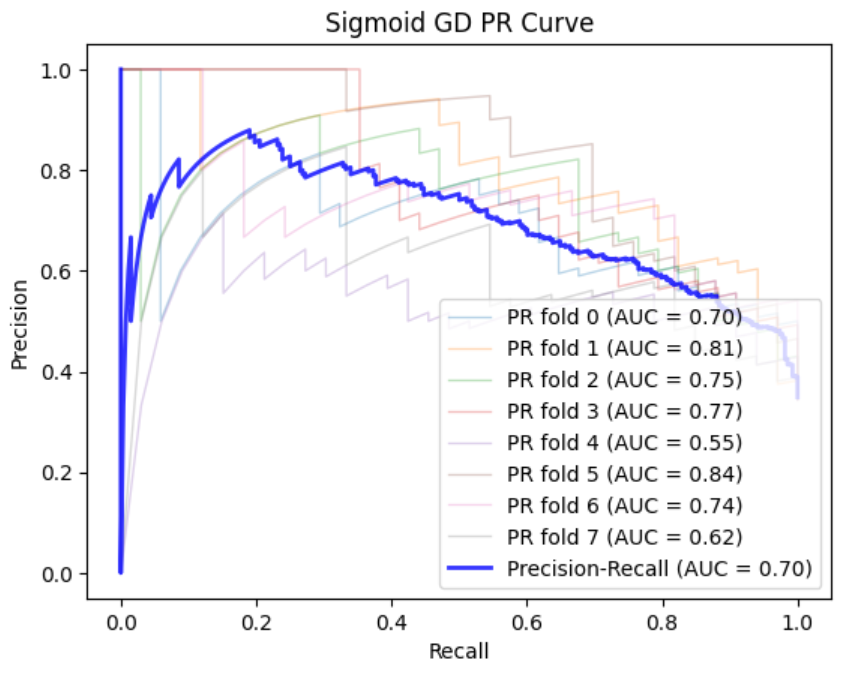
\includegraphics[width=0.5\textwidth]{images/gd_pr.png}
    \caption{Gradient Descent w/ Sigmoid Activation PR Curve.}
    \label{fig:gd_pr}
\end{figure}

The improvement in performance is likely due to the model being able to learn a more complex decision boundary. The sigmoid activation function allows the model to learn a non-linear decision boundary. Gradient descent also allows the model to learn more effectively by minimising the loss function rather than discreate updates like the Perceptron learning algorithm.

\subsection{Analysis}

The results of the models are summarised in Table \ref{tab:model_comparison}. The Gradient Descent w/ Sigmoid Activation model is the best performing model. It has the highest accuracy, F1 score, recall and precision. The mean PR AUC is also the highest of all the models. The model is able to learn a more complex decision boundary and is able to classify the positive class better than the other models.

What was not expected was that the Baseline w/ Bias model performed worse than the Baseline model. This was likely due to overfitting. The model was able to learn a decision boundary that was too closely fit to the training data. 


Other improvements that were attempted were using learning rate decay to train the GD model as well as using a tanh activation function and introducing stochasticity with batch updates. These did not improve the performance of the model and were not included in the final results.

Another experiment was performed to bias the positive class more by increasing the weight of the positive class. This did not improve the overall performance of the model but it did drastically increase the recall of the positive class. This could be useful in a real world scenario where we want to make sure that we are not missing any positive cases.


\section{Conclusion}
We explored multiple variations of a perceptron-based model for predicting diabetes using the Pima Indians Diabetes Database. Starting from a baseline perceptron model, we explored the addition of bias terms, L2 regularisation, class weighting, and then a more generalised model using gradient descent with sigmoid activation. Each modification provided insights into model behaviour with imbalanced datasets and demonstrated how tuning parameters such as learning rate and regularisation strength can impact overall performance as well as the limitations of the classic single layer perceptron model.

The best-performing model was the Gradient Descent with Sigmoid Activation, achieving a mean accuracy of 0.75 and an F1 score of 0.67, outperforming the other configurations. This improvement suggests that the ability to learn a non-linear decision boundary is crucial for the dataset's classification task.

The next steps could include exploring other training methods like ADAM or more complex architectures like multi-layer perceptrons or decision trees. Fine-tuning hyperparameters like class weights and incorporating advanced sampling techniques to address class imbalance could further improve model performance.

\clearpage

\begin{table}[ht!]
    \centering
    \resizebox{\textwidth}{!}{%
      \begin{tabular}{lccccc}
          \toprule
          \textbf{Model} & \textbf{Accuracy} & \textbf{F1 Score} & \textbf{Recall} & \textbf{Precision} & \textbf{Mean PR AUC} \\
          \midrule
          Baseline & 0.70 & 0.62 & 0.70 & 0.56 & 0.65 \\
          Baseline w/ Bias & 0.70 & 0.56 & 0.54 & 0.59 & 0.61 \\
          Baseline w/ Bias \& L2 Regularisation & 0.70 & 0.57 & 0.57 & 0.58 & 0.61 \\
          Baseline w/ Bias \& Class Weighting & 0.68 & 0.60 & 0.72 & 0.53 & 0.62 \\
          Gradient Descent w/ all & 0.75 & 0.67 & 0.72 & 0.62 & 0.71 \\
          \bottomrule
      \end{tabular}
    }
    \caption{Model Comparison}
    \label{tab:model_comparison}
\end{table}
